\begin{figure}
\begin{center}
    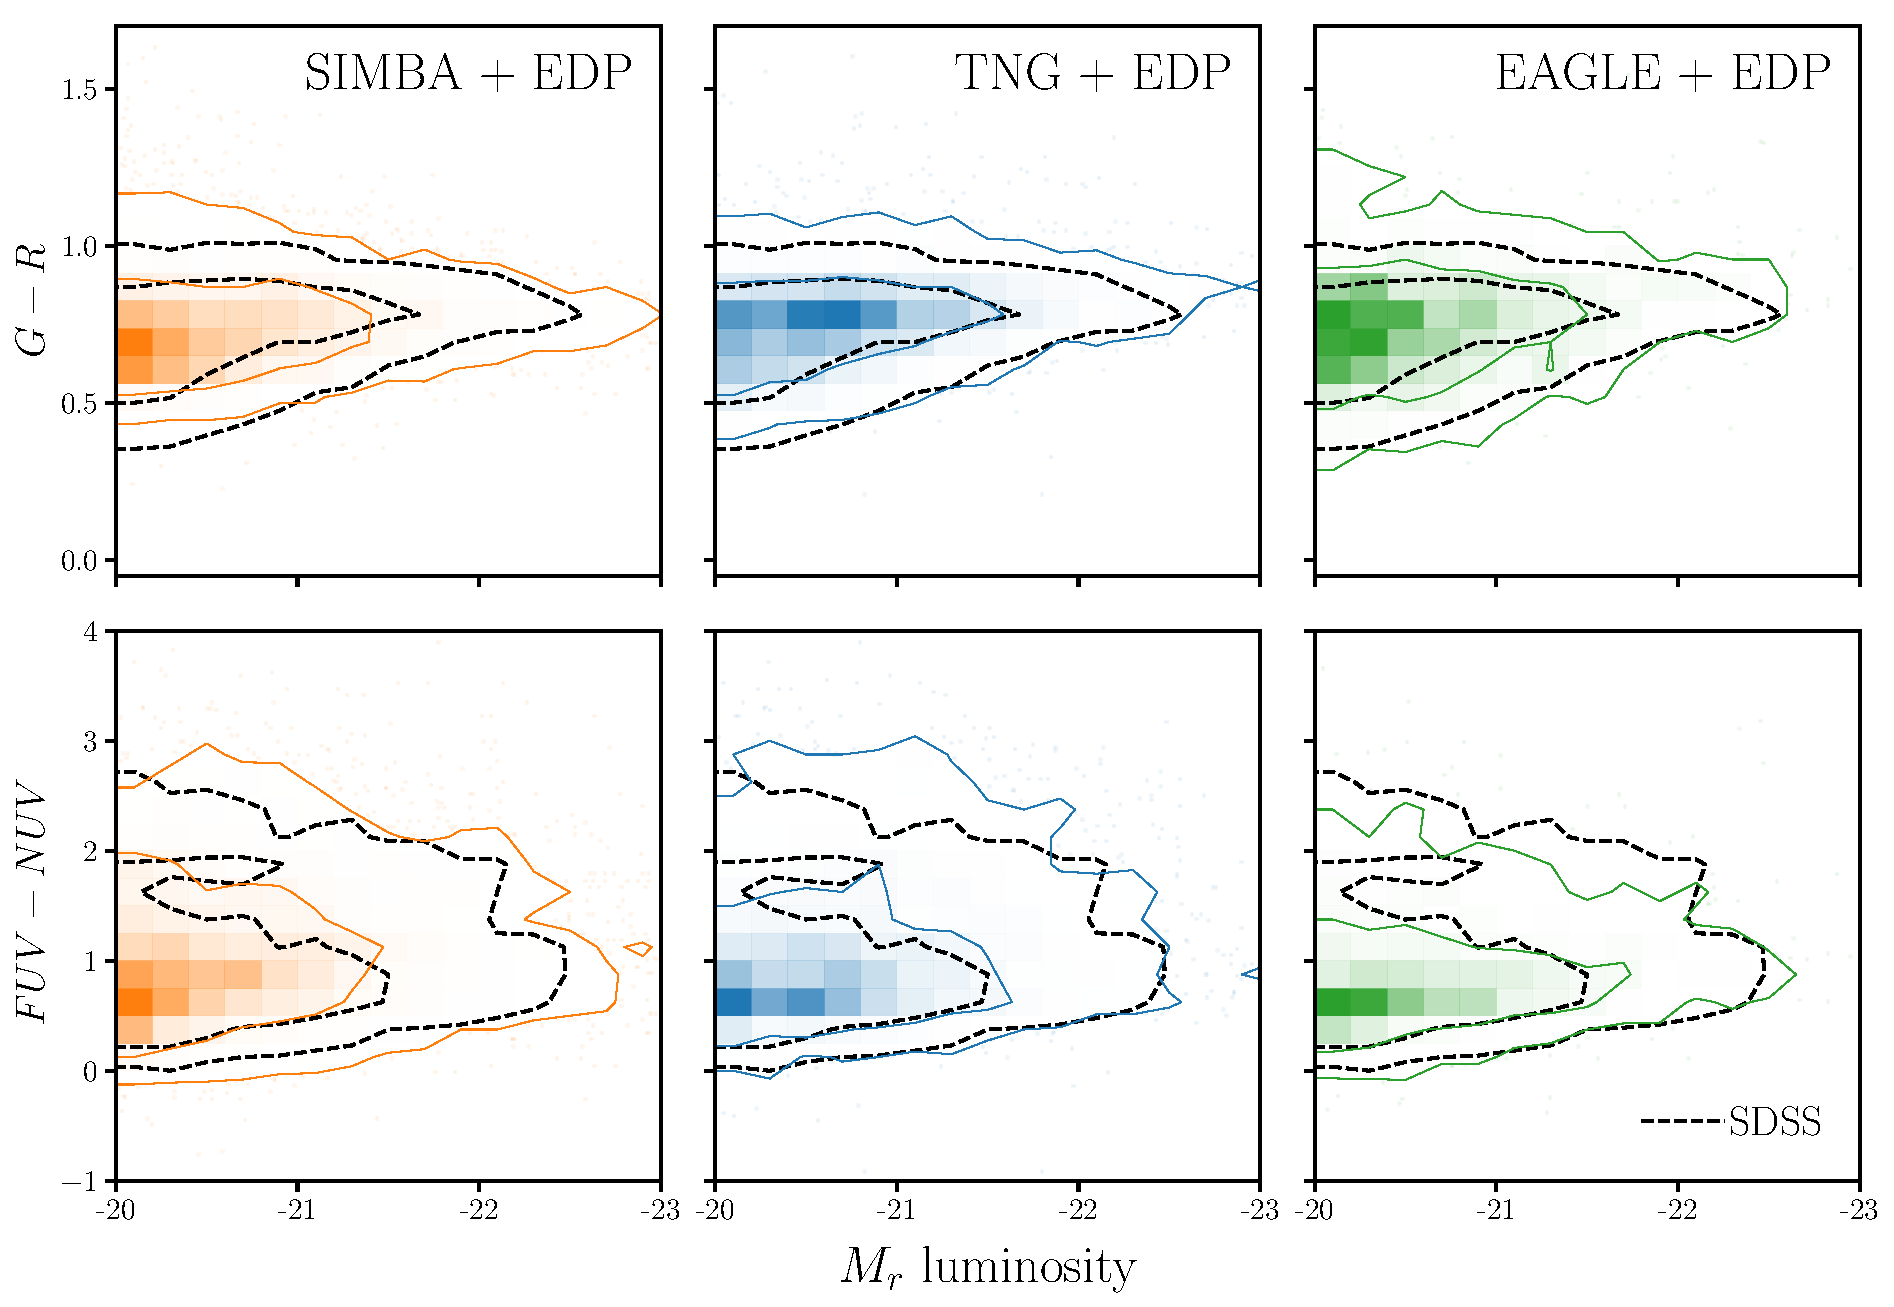
\includegraphics[width=0.9\textwidth]{figs/abc_observables.pdf}
    \caption{\label{fig:dem}
    The optical and UV color-magnitude relations predicted by the DEM with 
    the median ABC posteriors for the SIMBA (orange), TNG (blue), and EAGLE
    (green) hydrodynamical simulations. For comparison, we include the 
    $(\gr) - M_r$ (top panels) and $(\fnuv) - M_r$ (bottom panels) relations
    for SDSS (black dashed). With the DEM, the simulations produce dramatically 
    different observables than when we do not include any dust prescription
    (Figure~\ref{fig:obs}). Hence, dust must be account for when interpreting 
    and comparing simulations. Moreover, with the DEMs, all three simulations
    produce observables consistent with SDSS. Since different simulations can 
    produce reproduce observations by varying dust, dust significantly limits
    our ability to constrain the physical processes that go into galaxy
    simulations. 
    }
\end{center}
\end{figure}


%\begin{figure}
%\begin{center}
%    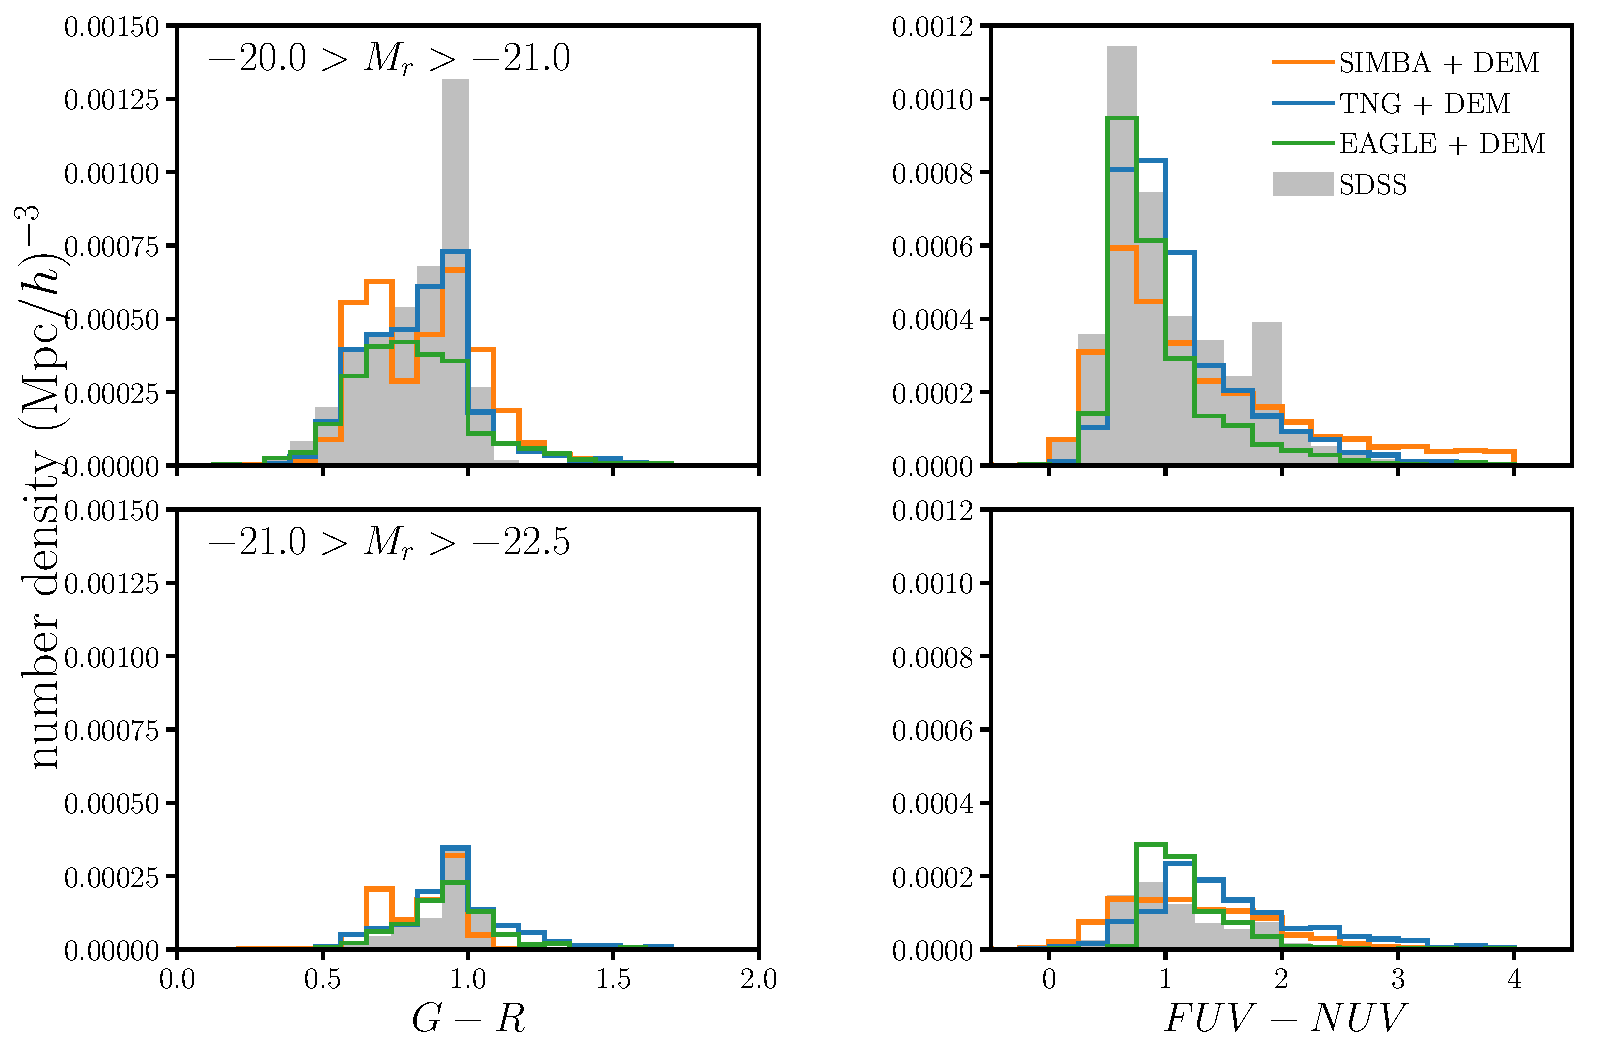
\includegraphics[width=0.85\textwidth]{figs/abc_observables_mr_bin.pdf}
%    \caption{\label{fig:demcloseup}
%    $G-R$ (left) and $FUV-NUV$ (right) number density distributions for the DEM
%    models of the SIMBA (orange), TNG (blue), and EAGLE (green) simulations in
%    two $M_r$ bins: $-20 > M_r > -21$ (top panels) and $-21 > M_r > -22.5$
%    (bottom panels).  Each of the DEM models are run using the median posterior
%    parameter values. In comparison to SDSS (grey shaded), the DEM models predict 
%    consistent red sequence and blue cloud positions in the $G-R$ distributions, 
%    $FUV-NUV$ peak positions, and number density. {\em Overall the DEM
%    models for SIMBA, TNG, and EAGLE produce observables are in good agreement 
%    with SDSS.}
%    }
%\end{center}
%\end{figure}


\section{Results} \label{sec:results}
In Figure~\ref{fig:dem}, we present the optical and UV color-magnitude
relations predicted by the DEM with the median ABC posteriors for the SIMBA
(orange), TNG (blue), and EAGLE (green) simulations. We include the SDSS
observables for comparison (black dashed). Without any dust attenuation, we
previously found that simulations predict dramatically different $(\gr) - M_r$
and $(\fnuv) - M_r$ relations than SDSS (Figure~\ref{fig:obs}). In contrast,
with the DEM, the optical color-magnitude relations have well-defined red
sequences and blue clouds that are consistent with SDSS. The DEM also produces
galaxies with $\fnuv$ distributions that are consistent with SDSS. We
also find good agreement in the galaxy number density at $M_r < -20$:
\ch{numbers} 

% comparison to literature 
% First EAGLE
Previous works in the literature have also compared colors and luminosities
predicted by simulations to observations. For EAGLE, \cite{trayford2015}
calculate colors and luminosities with the {\sc Galaxev} population synthesis
models and a two-component screen model for dust. More recently,
\cite{trayford2017} calculated optical colors for EAGLE using {\sc Skirt}, a
Monte Carlo radiative transfer code~\citep{camps2015}, to model the dust.
Both \cite{trayford2015} and \cite{trayford2017} produce bluer red sequences
compared to GAMA observations, at $10^{11.2} < M_* < 10^{11.5}$ for 
\cite{trayford2017}. Although a detailed comparison is difficult since both works
examine all galaxies, not only centrals, the DEM accurately reproduces the 
position of the SDSS red sequence, even at high $M_*$. \cite{trayford2015} 
also predict significant more luminous blue galaxies than obervations or the DEM. 
Using the same \cite{trayford2017} {\sc Skirt} framework, \cite{baes2019} find
that they overesimtate the observed cosmic spectral energy distributions 
(CSED) in the UV regime. Moreover, the $\fnuv$ color of their CSED is
significantly higher than GAMA $\fnuv$. The DEM, on the other hand, 
predict $\fnuv$ in good agreement with SDSS. 
%\cite{baes2019}: EAGLE+SKIRT SED compparison with GAMA Far UV is not attenuated enough. underrestimates optical and NIR
For TNG, \cite{nelson2018} calculate optical colors using a dust model that
includes attenuation due to dense gas birth clouds surrounding young stellar
populations and also due to simulated distribution of neutral gas and metals.
They find bluer red sequence peaks and a narrower blue cloud compared to SDSS.
Although they compare the color distribution for all galaxies in $M_*$ bins,
we find neither of these discrepancies with the DEM. 

Despite the success of the DEM, there are still some discrepancies with SDSS. 
For instance, the DEM produces broader distributions overall observations.
Central galaxies in SDSS sharply cut-off above the red sequence while some
galaxies in the DEM extend above this cut-off. The DEM color-magnitude
relations also extend more broadly to higher luminosities than SDSS. For SIMBA,
the DEM predicts a significant number of luminous ($M_r < -21$) blue galaxies 
not found in observations. Nonetheless, \emph{with the DEM, we produce optical
and UV color-magnitude relations that are in overall good agreement with
observations, better than previous works, for three different hydrodyanmical
simluations: SIMBA, TNG, and EAGLE.}

Figures~\ref{fig:dem} also highlights the fact that any comparison of
simulations must include dust attenuation. Dust dramatically changes the
predicted observables of simulations. Without dust (Figure~\ref{fig:obs}), we
did not find a clearly bimodality in the optical color-magnitude relation and
the simulations predicted UV colors outside of the range of observations.
But with a simple framework for dust motivated by attenuation laws and 
correlation with galaxy properties, such as the DEM, simulations can 
reproduce observations. 

These result highlights another key point. Robustly interpreting subgrid
physics in simulations requires marginalizing over dust. Even for three
simulations that produce significantly different SMFs and $M_*-\sfr$ relations
(Figure~\ref{fig:smf_msfr}), the DEM is able to produce observables that agree
with observations. In fact for SIMBA, the DEM reproduces the observations by assigning
higher attenuation to star-forming galaxies so that they populate the red sequence 
while quiescent galaxies populate the blue cloud. This is due to the large
number of low mass star-forming SIMBA galaxies that lie well above the SFS
(Figure~\ref{fig:smf_msfr}), which would otherwise all be luminous blue
galaxies not found in observations. Our current understanding of dust, which is
encapsulated in the DEM, has enough flexiblity to reproduce observations 
for simulations that predict galaxy populations with different physical
properties, even if it means contradicting the established relationship 
between color and $\sfr$. Then marginalizing over dust would leave little 
constraining power on the subgrid galaxy physics of the simulations. 
Therefore, \emph{current limitations in our understanding of dust in 
galaxies significant impedes our ability to investigate galaxy 
formation from simulations.}

% what we learn about AV - galaxy property connection  
In addition to reproducing observations, DEM also provides insight into dust in
galaxies. Given the parameterization of the DEM, it is especially easy to
interpret correlation between dust attenuation and galaxy physical properties.
In all three simulations, we find significant positive $M_*$ dependence of
$\tau_V$, $\mtaum \sim 2$ (Figure~\ref{fig:abc}), consistent with previous
works in the literature. \cite{burgarella2005}, for instance, found significant
positive $M_*$ dependence in $FUV$ attenuation in NUV-selected and FIR-selected
samples. \cite{garn2010} and \cite{battisti2016} also find positive $M_*$ 
dependence in SDSS star-forming galaxies. Most recently, \cite{salim2018} 
find higher $V$ and $FUV$ attenuation for more masssive star-forming galaxies in the
GALEX-SDSS-WISE Legacy Catalog 2 (GSWLC2). With the DEM we confirm that
\emph{galaxies with higher $M_*$ have overall higher dust attenuation}.
 %\todo{citation is a bit SDSS heavy.  Anything else in the literature?}

%\ch{SFR dependence of attenuation curves} 
In addition to the $M_*$ dependence, the DEM posteriors also reveal the
correlation between dust attenuation and star formation. We focus only on TNG
and EAGLE since SIMBA flips the color versus $\sfr$ relation. We infer DEM
posteriors with $\mtaus\sim-1$ --- galaxies with lower $\sfr$ have higher
attenuation. While observations have examined the relationship between dust
attenuation and $\sfr$~\citep[\eg][]{garn2010, reddy2015, battisti2016,
battisti2017}, they focus solely on star-forming galaxies. They find that
star-forming galaxies with higher SFR have higher attenuation; however, this
trend is driven by the $M_*$ dependence since star-forming galaxies lie on 
the star-forming sequence~\citep{garn2010, battisti2017}. At fixed $M_*$,
observations find no strong $\sfr$ dependence for the star-forming population. 
Since previous works do not include quiescent galaxies, the DEM provides new
insight into the $\sfr$ dependence of dust attenuation: \emph{quiescent
galaxies have overall higher dust attenuation}. 
%\cite{tress2018} find positive dependence between E(B-V) (color excess) with M* and negative dependence with
%SSFR for 1753 star-forming galaxies within 1.5 < z < 3.  

%For instance, \cite{garn2010} find that SDSS star-forming galaxies with higher
%SFR have higher H$\alpha$ attenuation. \cite{battisti2016} find a consistent
%correlation for the Balmer optical depth of star-forming galaxies in GALEX and SDSS 
%using 10000 SF galaxies GALEX-SDSS. Although at higher redshifts,  
%\cite{reddy2015} also find this correlation among $z{\sim}2$ star-forming galaxies of
%MOSFIRE Deep Evolution Field.

%\cite{battisti2017} using 5000 SF galaxies from found little stellar mass dependence in the opposite direction (less attenuation at higher stellar masses). But they have big error bars and only probe up to 9.7
%\cite{reddy2015} SF galaxies from $z\sim2$ MOSFIRE Deep Evolution Field survey find strong correlation with SFR. %ionized gas is more reddened relative to the stellar continuum with increasing SFR 

\begin{figure}
\begin{center}
    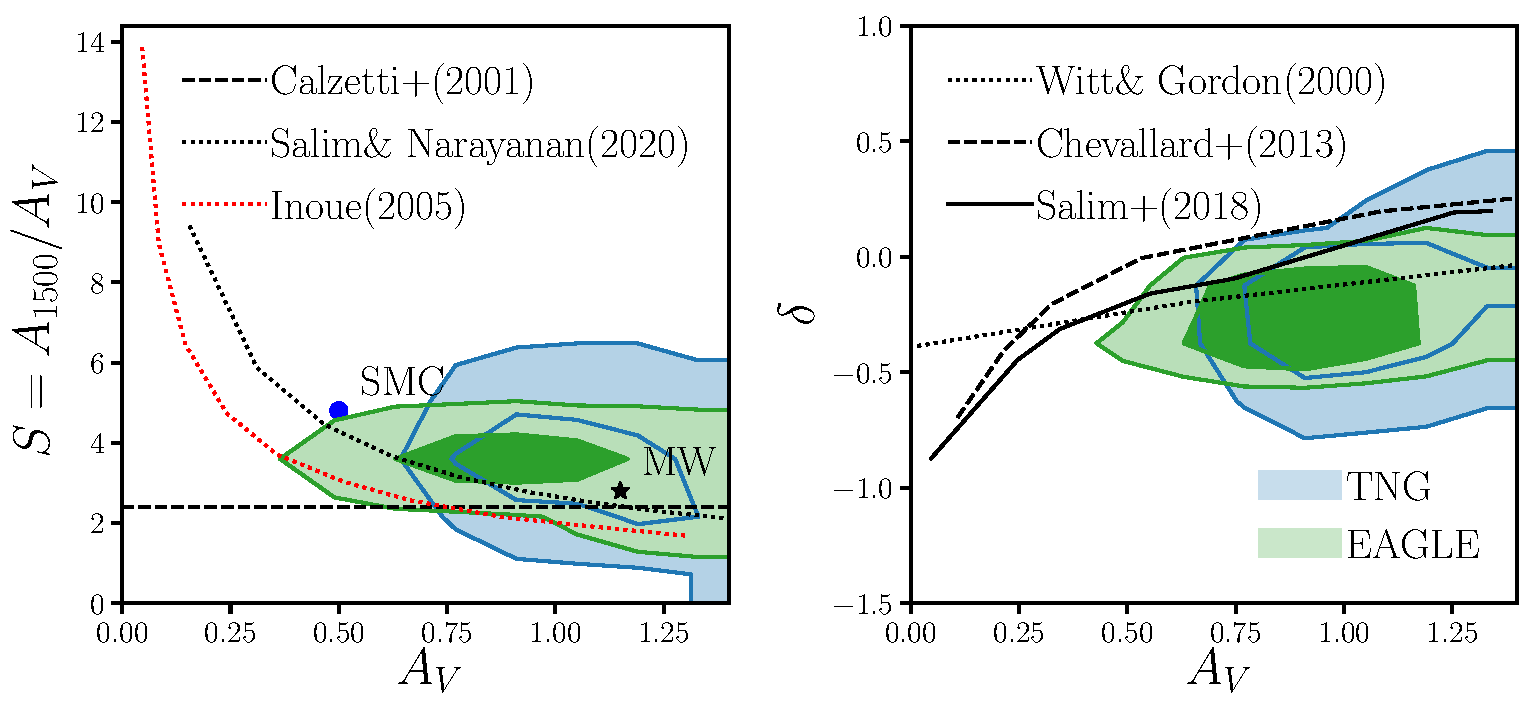
\includegraphics[width=0.85\textwidth]{figs/abc_slope_AV.pdf}
    \caption{\label{fig:slope}
    The attenuation-slope relation for TNG (blue) and EAGLE (green) simulations
    with the DEM. We present the relation usng two different measurements of slope, 
    commonly used in the ltierature: $S = A(1500\AA)/A_V$ (left panel) and
    the slope offset from the \cite{calzetti2001} curve, $\delta$ (right panel).
    The DEM moodels predict an attenuation-slope relation, where the slope is
    steeppr at lower attenuation, consistent with both observations and
    simulation. The DEM models only include masssive galaxies, hence, they do
    not include mnay galaxies with low attenuatiton. At $A_V > 0.5$, however, 
    the DEM models are in good agreement with observations~\cite{salim2020}. In
    fact, the DEM models match the observed attenuation-slope relation 
    better than radiative transfer simulations, which predict attenuation 
    curves that are too shallow~\citep{inoue2005, chevallard2013, trayford2020}
    }
\end{center}
\end{figure}

% attenuation curve slope  
Our results also shed light on the slope of dust attenuation and its
correlation to galaxy properties. In Figure~\ref{fig:slope}, we present the
attenuation-slope relation for TNG (blue) and EAGLE (green) with the DEM. The
left and right panels present two different measurements of the slope $S =
A(3000\AA)/A_V$, which is easier to cosntrain in observations, and $\delta$,
the slope offset from the \cite{calzetti2001} curve that use in the DEM. 
We include the attenuation and lsope for the Milky Way (star) for reference.
TNG and EAGLE both predict slopes within $2 < S < 5$ and centered around $S\sim
3.5$. In comparison, \cite{leja2017} and \cite{salim2018} find a broader range 
of slopes in their galaxy samples, $2 < S < 15$. However, this is because their
sample includes galaxies with $A_V < 0.4$ that have steeper slopes. Excluding
these galaxies, which are not in our sample, we find good agreement with 
\cite{leja2017} and \cite{salim2018}. Other observations find slopes within 
the range $2 < S < 5$ for star-forming galaxies~\citep{calzetti2000, burgarella2005, johnson2007,
conroy2010, wild2011, battisti2016, battisti2017}. Therefore, \emph{the dust
attenuation curve slopes predicted by the DEM for TNG and SIMBA are in
excellent overall agreement with observations}. 

%\cite{calzetti2000} find  slopes of $2.3 < S < 2.9$ for low-redshift starburst galaxies, 
%\cite{burgarella2005} find $2.5 < S < 6.2$ for 50 UV and 100 IR selected galaxies,
%\cite{johnson2007} find $S\sim2.5$ for 1000 nearby galaxies, 
%\cite{conroy2010} find $S\sim4.5$ for 3400 $10^{9.5} < M_* < 10^{10} M_\odot$ disk galaxies,
%\cite{wild2011} find $2.5 < S < 4.5$ for 23,000 $z{\sim}0.07$ star-forming galaxies, 
%\cite{battisti2016, battisti2017} find slopes consistent with Calzetti (S=2.4) for SF galaxies 
%\cite{leja2017} 130 relatively massive galaxies 2 < S < 15
%\cite{salim2018} 230,000 SDSS galaxies 2 < S < 15 with median S = 5.4
% high z
%\cite{kriek2013}  using stacked SEDs of medium- and broadband photometry of
%galaxies at 0.5 < z < 2 find an average slope of delta=-0.2  but they restrict
%to galaxies with moderate to high optical attenuations (AV> 0.5), 
%\cite{salmon2016} is also spot on. 

With the DEM, we can also examine the correlation between attenuation curve
slopes and galaxy properties. For TNG and EAGLE, we find that the slope of the
attenuation curve does not depend significantly on $M_*$ or $\sfr$.
\cite{leja2017} find composite and AGN galaxies generally have shallower  
slopes, although their sample is limited to only 129 galaxies, In contrast,
\cite{salim2018} find that quiescent galaxies in the GALEX-SDSS-WISE Legacy
Catalog 2~\citep[GSWLC2;][]{salim2019} have significantly steeper curves. They,
however, also find significantly steeper curves for the starburst population 
(\ie~galaxies above the SFS). With no consensus in the literature and few
observations that examine the correlation between $\delta$ and galaxy
properties, the lack of $M_*$ and $\sfr$ dependence we find on $\delta$ is an
interesting prediction for future observations. 

% attenuation-slope relation 
Next, we examine the attenuation-slope relation. At low attenuation, dust scattering dominates absoprtion. In this regime,
the attenuation curve steepens because red light tends to
scatter isotropically while blue light tends to forward scatter, which causes
more optical-to-IR light to escape the galaxy than UV light~\citep{gordon1994,
witt2000, draine2003}. On the other hand, at high attenuation dust absorption 
is dominant and the attenuation curve is shallower~\citep{chevallard2013}.
In both panels of Figure~\ref{fig:slope}, the DEM predicts attenuation--slope
relations where the slope is steeper at lower attenuation. Furthermore, for the
$A_V$ range probed by the DEM, the DEM $A_V$--slope relations are consistent with 
the $A_V - S$ relation of GSWLC2 galaxies~\citep[black shaded][]{salim2020}.
They are also consistent with \cite{leja2017}. 
We also compare our results to theoretical predictions from radiative transfer
models~\citep{inoue2005, chevallard2013, trayford2020}. \cite{inoue2005}
(dotted), the radiative transfer models considered in \cite{chevallard2013}
(dot dashed), and \cite{trayford2020} (light shaded) all predict shallower 
attenuation curves than observations. This is also the case for the
\cite{narayanan2018} attenuation curves, not included in Figure~\ref{fig:slope}. 
Therefore, the DEM not only predicts the established attenuation--slope relation, 
but it also better reproduces the observations than radiative transfer models. 

%\cite{trcka2020}: EAGLE+SKIRT with CIGALE to get physical properties of
%galaxies. trcka2020 compares to dustpedia~\citep{davies2017} They lok at
%IRX-beta relation.

\begin{figure}
\begin{center}
    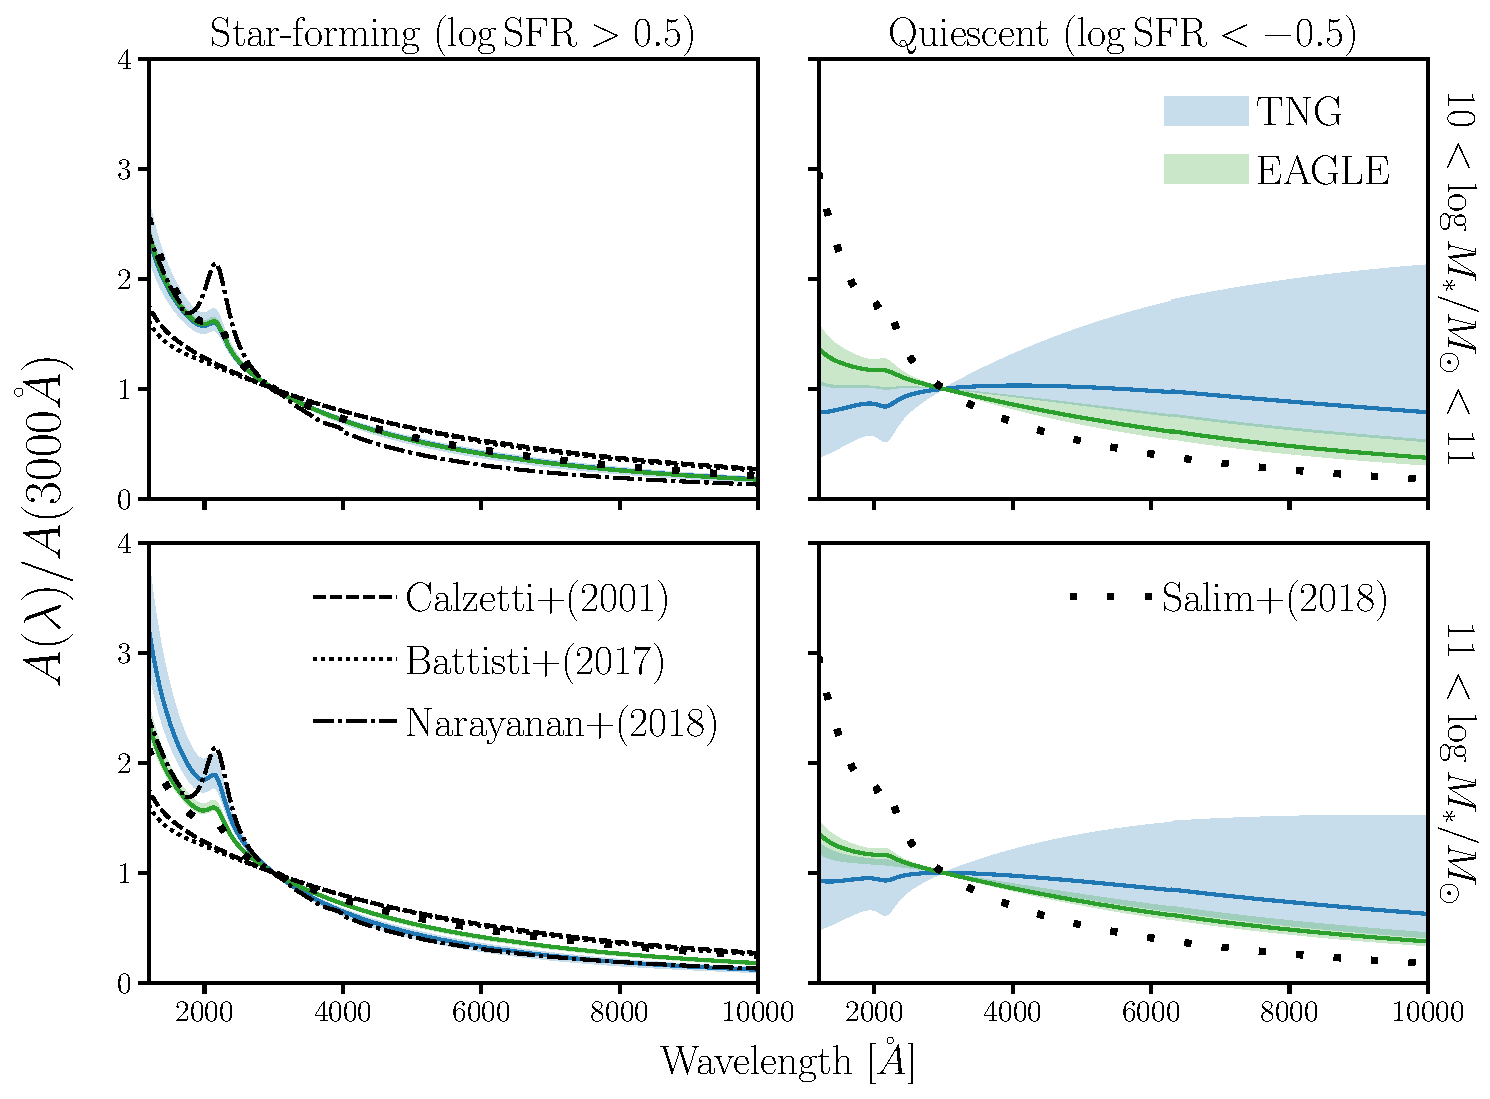
\includegraphics[width=0.85\textwidth]{figs/abc_attenuation.pdf}
    \caption{\label{fig:atten}
    Attenuation curves of the TNG (blue) and EAGLE (green) DEM models for 
    low (top) and high $M_*$ (bottom), star-forming (left) and
    quiescent galaxies (right). The attenuation curves are normalized at
    $3000\AA$: $A(\lambda)/A(3000\AA)$. We mark the $1\sigma$ standard
    deviation of the attenuation curves with the shaded region. For comparison,
    we include measurements of $A(\lambda)/A(3000\AA)$ from 
    observations~\citep{caleztti2000, battisti2017, salim2018} as well as
    from simulations~\citep{narayanan2018}. For star-forming galaxies, the 
    \cite{calzetti2000} and \cite{battisti2017} attenuation curves are shallower 
    than the DEM attenuation curves; however, this is primarily driven by the
    differences in $M_*$ ranges. For \cite{salim2018}, which probe a similar
    $M_*$ range as our DEM models, we find goood agreement. We also find good 
    agreement with median attenuation curve of \cite{narayanan2018}. With DEM
    models, we can also constrain the attenuation curves of quiescent galaxies,
    which are challenging to observationally constrain. Quiescent galaxies,
    have significantly shallower attenuation curves with larger variations in
    slope. 
    }
\end{center}
\end{figure}

% variation of attenuation curve  
Although the DEM does not explicitly model the complexities of dust-star geometry on a
galaxy-by-galaxy basis, through the slab model and the dependence on galaxy
properties, it includes significant variations in the dust attenuation. In
Figure~\ref{fig:atten}, we present the normalized attenuation curves of the TNG
(blue) and EAGLE (green) DEM for low (top) and high $M_*$ (bottom),
star-forming (left) and quiescent galaxies (right).  The attenuation curves are
normalized at $3000\AA$: $A(\lambda)/A(3000\AA)$. The variation in the
attenuation curves (1$\sigma$ standard deviation about the median) is
represented by the shaded region. For comparison, we include
$A(\lambda)/A(3000\AA)$ from observations~\citep{calzetti2000, battisti2017, salim2018} 
as well as from simulations~\citep{narayanan2018}. The \cite{calzetti2000} and
\cite{battisti2017} attenuation curves are for star-forming galaxies with
significantly lower $M_*$. The \cite{battisti2017} curve, for instance, is
derived from $M_* < 10^{9.9}M_\odot$ star-forming galaxies. Meanwhile, the
\cite{salim2018} curves we include are specifically for $10^{9.5} < M_* < 10^{10.5}M_\odot$ 
star-forming galaxies (top left), $10^{10.5} < M_*M_\odot$ star-forming
galaxies (bottom left), and quiescent galaxies (top and bottom right panels). 


Focusing first on the attenuation curves of star-forming galaxies (left
panels), we find that the \cite{calzetti2000} and \cite{battisti2017} curves
are significantly shallower than the TNG and EAGLE DEM attenuation curves.
Part of this discrepancy is driven by differences in $M_*$. Although we do not
probe to low $M_*$, since the TNG and EAGLE attenuation curves get shallower at
lower $M_*$, we expect better agreement with \cite{calzetti2000} and
\cite{battisti2017} at the $M_*$ ranges they probe. 
Next, compared to \cite{salim2018}, we find good agreement among the attenuation
curves for star-forming galaxies. Furthermore, the variation in the DEM attenuation curves of star-forming galaxies is consistent with the
variation in Figure 9 of \cite{salim2018}. The DEM attenuation
curves are also in excellent agreement with the median attenuation curve of
\cite{narayanan2018} star-forming galaxies. While \cite{narayanan2018} find
larger variations than the DEM, this is in part because of their broader $M_*$ 
range. Hence, \emph{for star-forming, the DEM find significant variation in dust 
attenuation consistent with both observations and simulations.}

%\ch{what do we learn about quiescent galaxy attenuation?} 
The DEM also sheds light on dust attenuation in quiescent galaxies. This is
particularly valuable since there are many challenges to measuring attenuation
curves for quiescent galaxies in observations. For instance, methods that rely
on IR luminosities can be contaminated by MIR emission from AGN heating nearby
dust~\cite{kirkpatrick2015}. Even SED fitting methods require accounting for
AGN MIR emission~\citep{salim2016, leja2018, salim2018} in addition to the
challenge in breaking the degeneracy between SFH and metallicity to fit the
continuum (\ch{cite?}). With the DEM, which foward models optical and UV
photometry, we do not face these issues. For both TNG and EAGLE, quiescent
galaxies have shallower attenuation curve with large variations in the slopes
(Figure~\ref{fig:atten}). They also have higher $A_V \gtrsim 1.25$. 
\ch{explanation for why DEM model does this} 

%In \cite{leja2017}, they similar find composite and AGN galaxies
%to have shallow attenuation curves with higher $A_V$; however, the comparison
%is limited due to ther smaller sample size (129 galaxies). In contrast,  
%\cite{salim2018} find that quiescent galaxies in GSWLC2 have significantly
%steeper curves; they, however, focus their analysis mainly on star-forming 
%galaxies.

% Kartheik on why dust is hard to constrain for quiescent galaxies: 
%firstly because quiescent galaxies don't have much recent SFR and therefore not much dust (their most recently produced dust has likely happened more than a dust destruction timescale ago), 
% secondly because the continuum for quiescent galaxies is super hard to fit (and break degeneracies with SFH & metallicity), which leads to poor(er) constraints. You could basically think of this in terms of dust/total SNR, which drops sharply for this population.

In our DEM model, we neglect the galaxies with SFR=0 from simulations by
directly sampling the quiescent galaxy observables (Section~\ref{sec:res}).
Since galaxies with SFR=0 predicted by the simulations do not have recent 
star-formation and also have 0 gas mass\todo{@tjitske is this for all
sims}, we would expect them to also have no dust. However, a DEM model
where we do not attenuate SFR=0 galaxies struggles to reproduce observations.
This likely highlights the limitations of hydrodynamical simulations near the
mass and temporal resolutions as well as the limitations of subgrid
prescriptions for gas. \ch{Uncertainties in the dust desctruction timescale may
also contribute to the explanation~\citep[\eg][]{jones2011, slavin2015}}. 
We emphasize that our prescription for SFR=0 galaxies ensures that they do not
significantly impact the constraints on DEM parameters. 



For the DEM model in this paper, we fix the amplitude of the UV dust bump to
the amplitude of $\delta$ (Eq.~\ref{eq:bump_amp}). If, rather than fixing $m_E$ and
$c_E$ in Eq.~\ref{eq:bump_amp}, we allow them to be free parameters we find
litte constraing power on these parameters. More importantly, we find
consistent constraints for the other DEM parameters, which implies that fixing
the UV bump parameters does not impact our results. 

A major assumption in the DEM model is how we sample the $A_V$ using the slab
model. For each simulated galaxy, the DEM model uniformly samples the
inclination and then assigns $A_V$ with the slab model (Eq.~\ref{eq:slab}). As
we detail in Section~\ref{sec:dem}, this slab model is consistent inclination
dependence of attenuation found in both observations~\citep[\eg][]{conroy2010,
salim2020} and simulations~\citep[\eg]{chevallard2013, narayanan2018,
trayford2020}. Moreover, the slab model successfully reproduces the $A_V$
distribution of SDSS galaxies (Figure~\ref{fig:av_dist}). To ensure that our
results do not hinge on the slab model, we conduct our analysis using a
a truncated normal distribution based DEM model to sample $A_V$
(Appendix~\ref{sec:nonslab}). This model is more flexible than the slab model. 
For instance, we include physical parameter dependence for the scatter of
$A_V$, and not just for $\tau_V$. We refer readers to Appendix~\ref{sec:nonslab} for details. 
We find that adding our results are not impacted by the change in the $A_V$ 
sampling model or the added flexiblity. Therefore, our results are not driven
by our choice of the slab model. 

% Salim(2020): Chevallard et al. (2013), who aggregated and analyzed a diverse series of theoretical attenuation law studies by Pierini et al. (2004), Tuffs et al. (2004), Silva et al. (1998) and Jonsson et al. (2006), and showed that all the stud- ies predict, with some normalization differences, a relationship between the optical depth AV and attenuation law slope.

% Salmon+(2016): There is evidence that galaxy inclination correlates with the strength of Lyα emission, such that we observe less Lyα equivalent width for more edge-on galaxies (Charlot & Fall 1993; Laursen & Sommer-Larsen 2007; Yajima et al. 2012; Verhamme et al. 2012; U et al. 2015)
% Therefore, based on physi- cal models, one expects that galaxies with “greyer” dust laws and larger overall attenuation should have higher inclinations
% Salim+(2018): Chevallard et al. (2013) furthermore show that the depend- ence of the slope on AV is the same irrespective of whether the AV is driven by different levels of intrinsic (face-on) attenuation or is the result of inclined viewing geometry. 

\ch{How about our prior choice?}

% recap everything
\ch{what we learn about in the simulations}


\ch{what we learn about dust}  
paragraph on restating how we can learn about dust through DEMs based on trends we see
across all simulations. summarize main findings again. 

\ch{observables unaffected by dust/dem?}
Are there observables that hydro sims + DEMs cannot reproduce? What does that say about the hydro sims?
What observables are unaffected by DEMs? We should chase those observables. 

\ch{don't over-interpret observations}
We clearly have to becareful with overinterpreting hydro sims because modifying
dust allows us to reproduce whatever we want. 
\begin{itemize}
    \item Should we bother calibrating our empirical and semi-analytic models
        to hydrodynamic simulations when the hydro sims also require
        marginalizing over dust parameters? Does this mean that if our goal is
        to make realistic mocks, we can be relatively careless about 
\end{itemize}

\ch{What are some applications for DEMs?}
Realistic mock catalogs that reproduce observations in observable-space rather
than physical parameter space. \ch{talk about IQ paper where we use best-fit
dust}  
